\section{Struttura del blueprint}\label{s:struttura-blueprint}
La realizzazione del blueprint è avvenuta in diverse iterazioni. Nella seguente sezione descriviamo, in ordine cronologico, come siamo giunti alla versione finale.

\subsection{Componenti utilizzate}\label{ss:componenti-utilizzate}
Nelle varie pagine vengono sfruttate delle tipologie di componenti che si è soliti trovare nelle dashboard. Di seguito ne presentiamo l'utilizzo che ne abbiamo fatto noi:
\begin{itemize}
    \item \textbf{box con indicatore numerico}: mostrano principalmente valori numerici con un'etichetta che li indica, all'interno di un riquadro. È stato utilizzato per proprietà dei concetti come: nuovi positivi, nuovi decessi, nuovi ingressi in terapia intensiva, e molti altri;
    \item \textbf{box con grafico seriale}: mostrano serie numeriche sotto forma di grafici per illustrare l'andamento di determinate curve basate sui dati temporali;
    \item \textbf{box con diagramma a barre}: descrive la distribuzione doppia di una metrica;
    \item \textbf{box con mappa}: mostra la mappa dell'Italia o di una regione, a tinta unita o come \textit{heat map}, per avere il colpo d'occhio sulla situazione;
    \item \textbf{box con indicatori di livello}: mostra dei valori di certe proprietà sotto forma d'indicatori di livello, altresì detti \textit{gauge}, per evidenziare quando una proprietà numerica si trova in un range preoccupante, intermedio o tranquillo in un modo grafico immediato. Ad esempio, il tasso di positività può ritenersi preoccupante sopra il 15\% (indicatore su zona rossa), intermedio fra il 10\% e il 15\% (indicatore su zona gialla), tranquillo sotto il 10\% (indicatore su zona verde);
    \item \textbf{box con lista di elementi}: mostra certe proprietà sotto forma di liste di elementi, per esempio il totale degli attuali positivi per ogni regione;
    \item \textbf{box con areogramma}: mostra una cerchio diviso in sezioni, ciascuna di esse rappresenta la proporzione sul totale di una proprietà di un concetto;
    \item \textbf{box con tabella}: mostra una tabella; è utilizzato per visualizzare i valori delle metriche per ogni regione o provincia, le righe sono ordinabile in maniera crescente/decrescente in base ad una delle metriche che si trovano sulle colonne.
\end{itemize}

\subsubsection{Prima iterazione}
\begin{figure}[H]
    \centering
    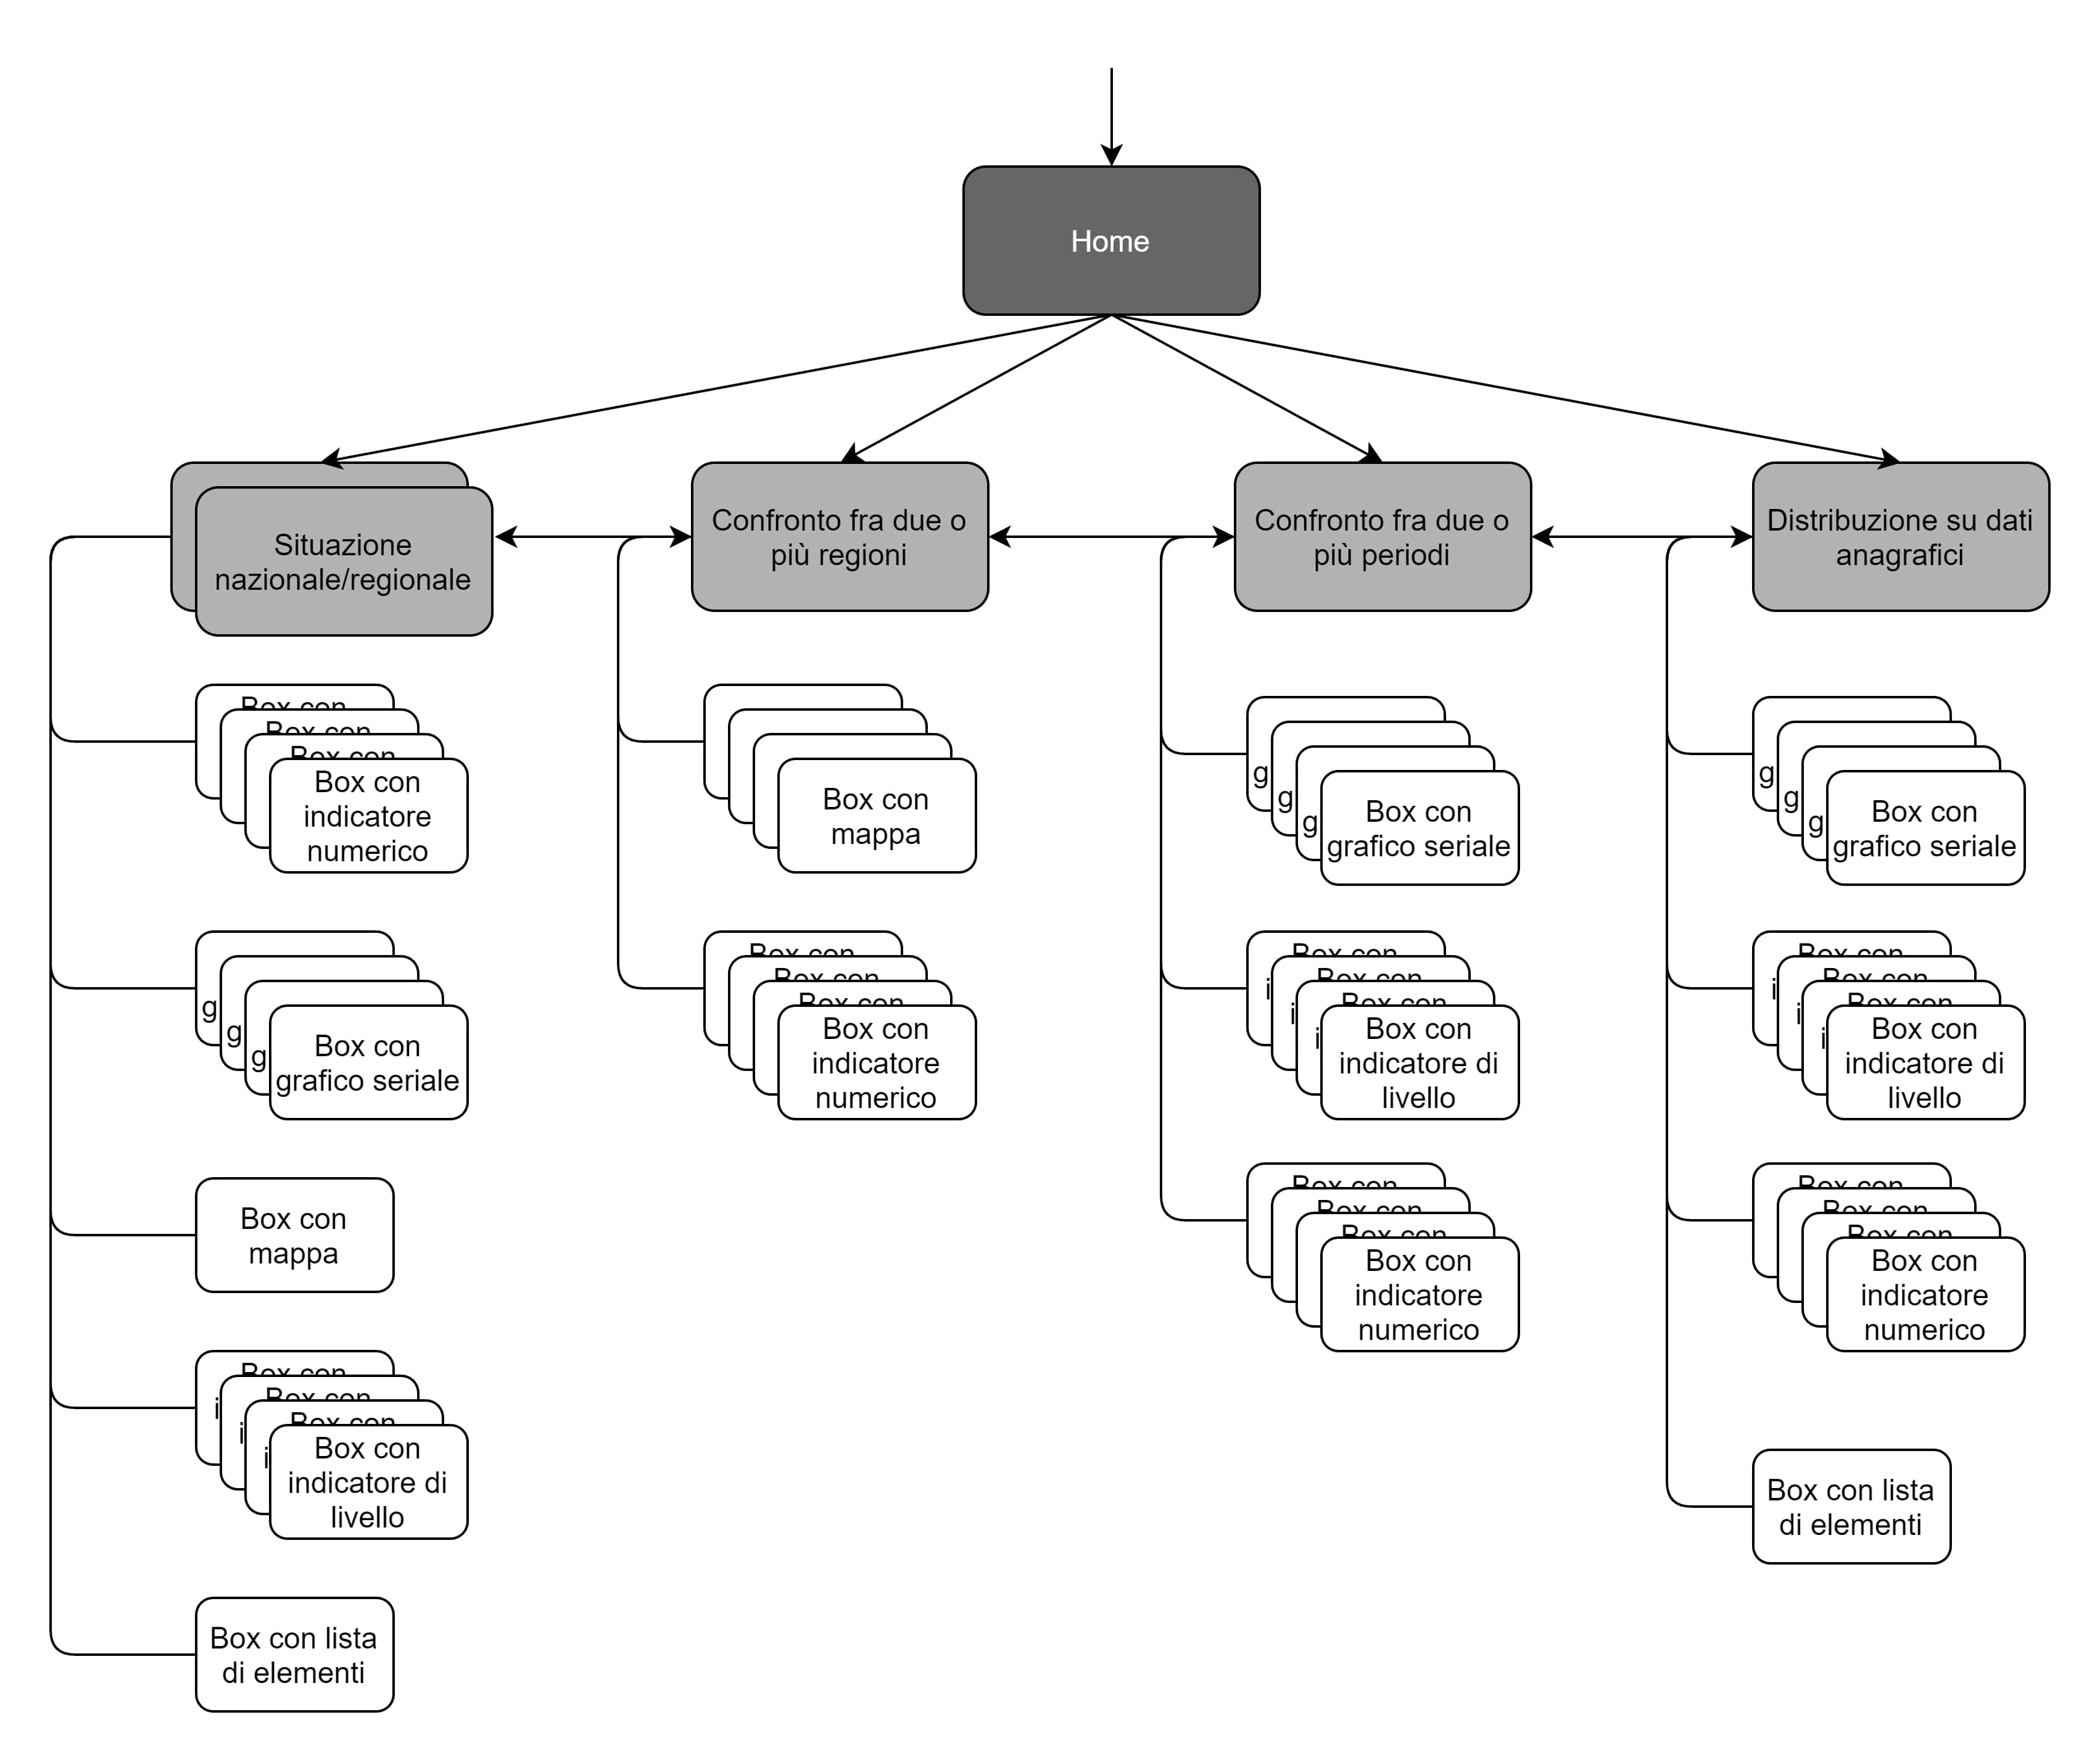
\includegraphics[width=1.0\columnwidth]{structure-blueprint/blueprint-prog-1}
    \caption{Prima versione del blueprint.}\label{fig:blueprint-prog-1}
\end{figure}
Diversamente da quanto avviene nella dashboard del DPC attuale, avevamo inizialmente pensato che la home page potesse essere una semplice pagina che permettesse la scelta fra le quattro pagine indicate:
\begin{itemize}
    \item Situazione nazionale/regionale: due pagine simili ma con contenuto riferito l'una all'intera nazione, l'altra a una singola regione;
    \item Confronto fra due o più regioni;
    \item Confronto fra due o più periodi;
    \item Distribuzione sui dati anagrafici.
\end{itemize}
Ci siamo immediatamente resi conto che questa modalità sarebbe stata scarsamente pratica poiché già all'avvio della dashboard l'utente non avrebbe avuto il ``colpo d'occhio'', potenzialmente penalizzandola. Abbiamo quindi modificato quanto prodotto raggiungendo una seconda versione del blueprint.

\subsubsection{Seconda iterazione}
\begin{figure}[H]
    \centering
    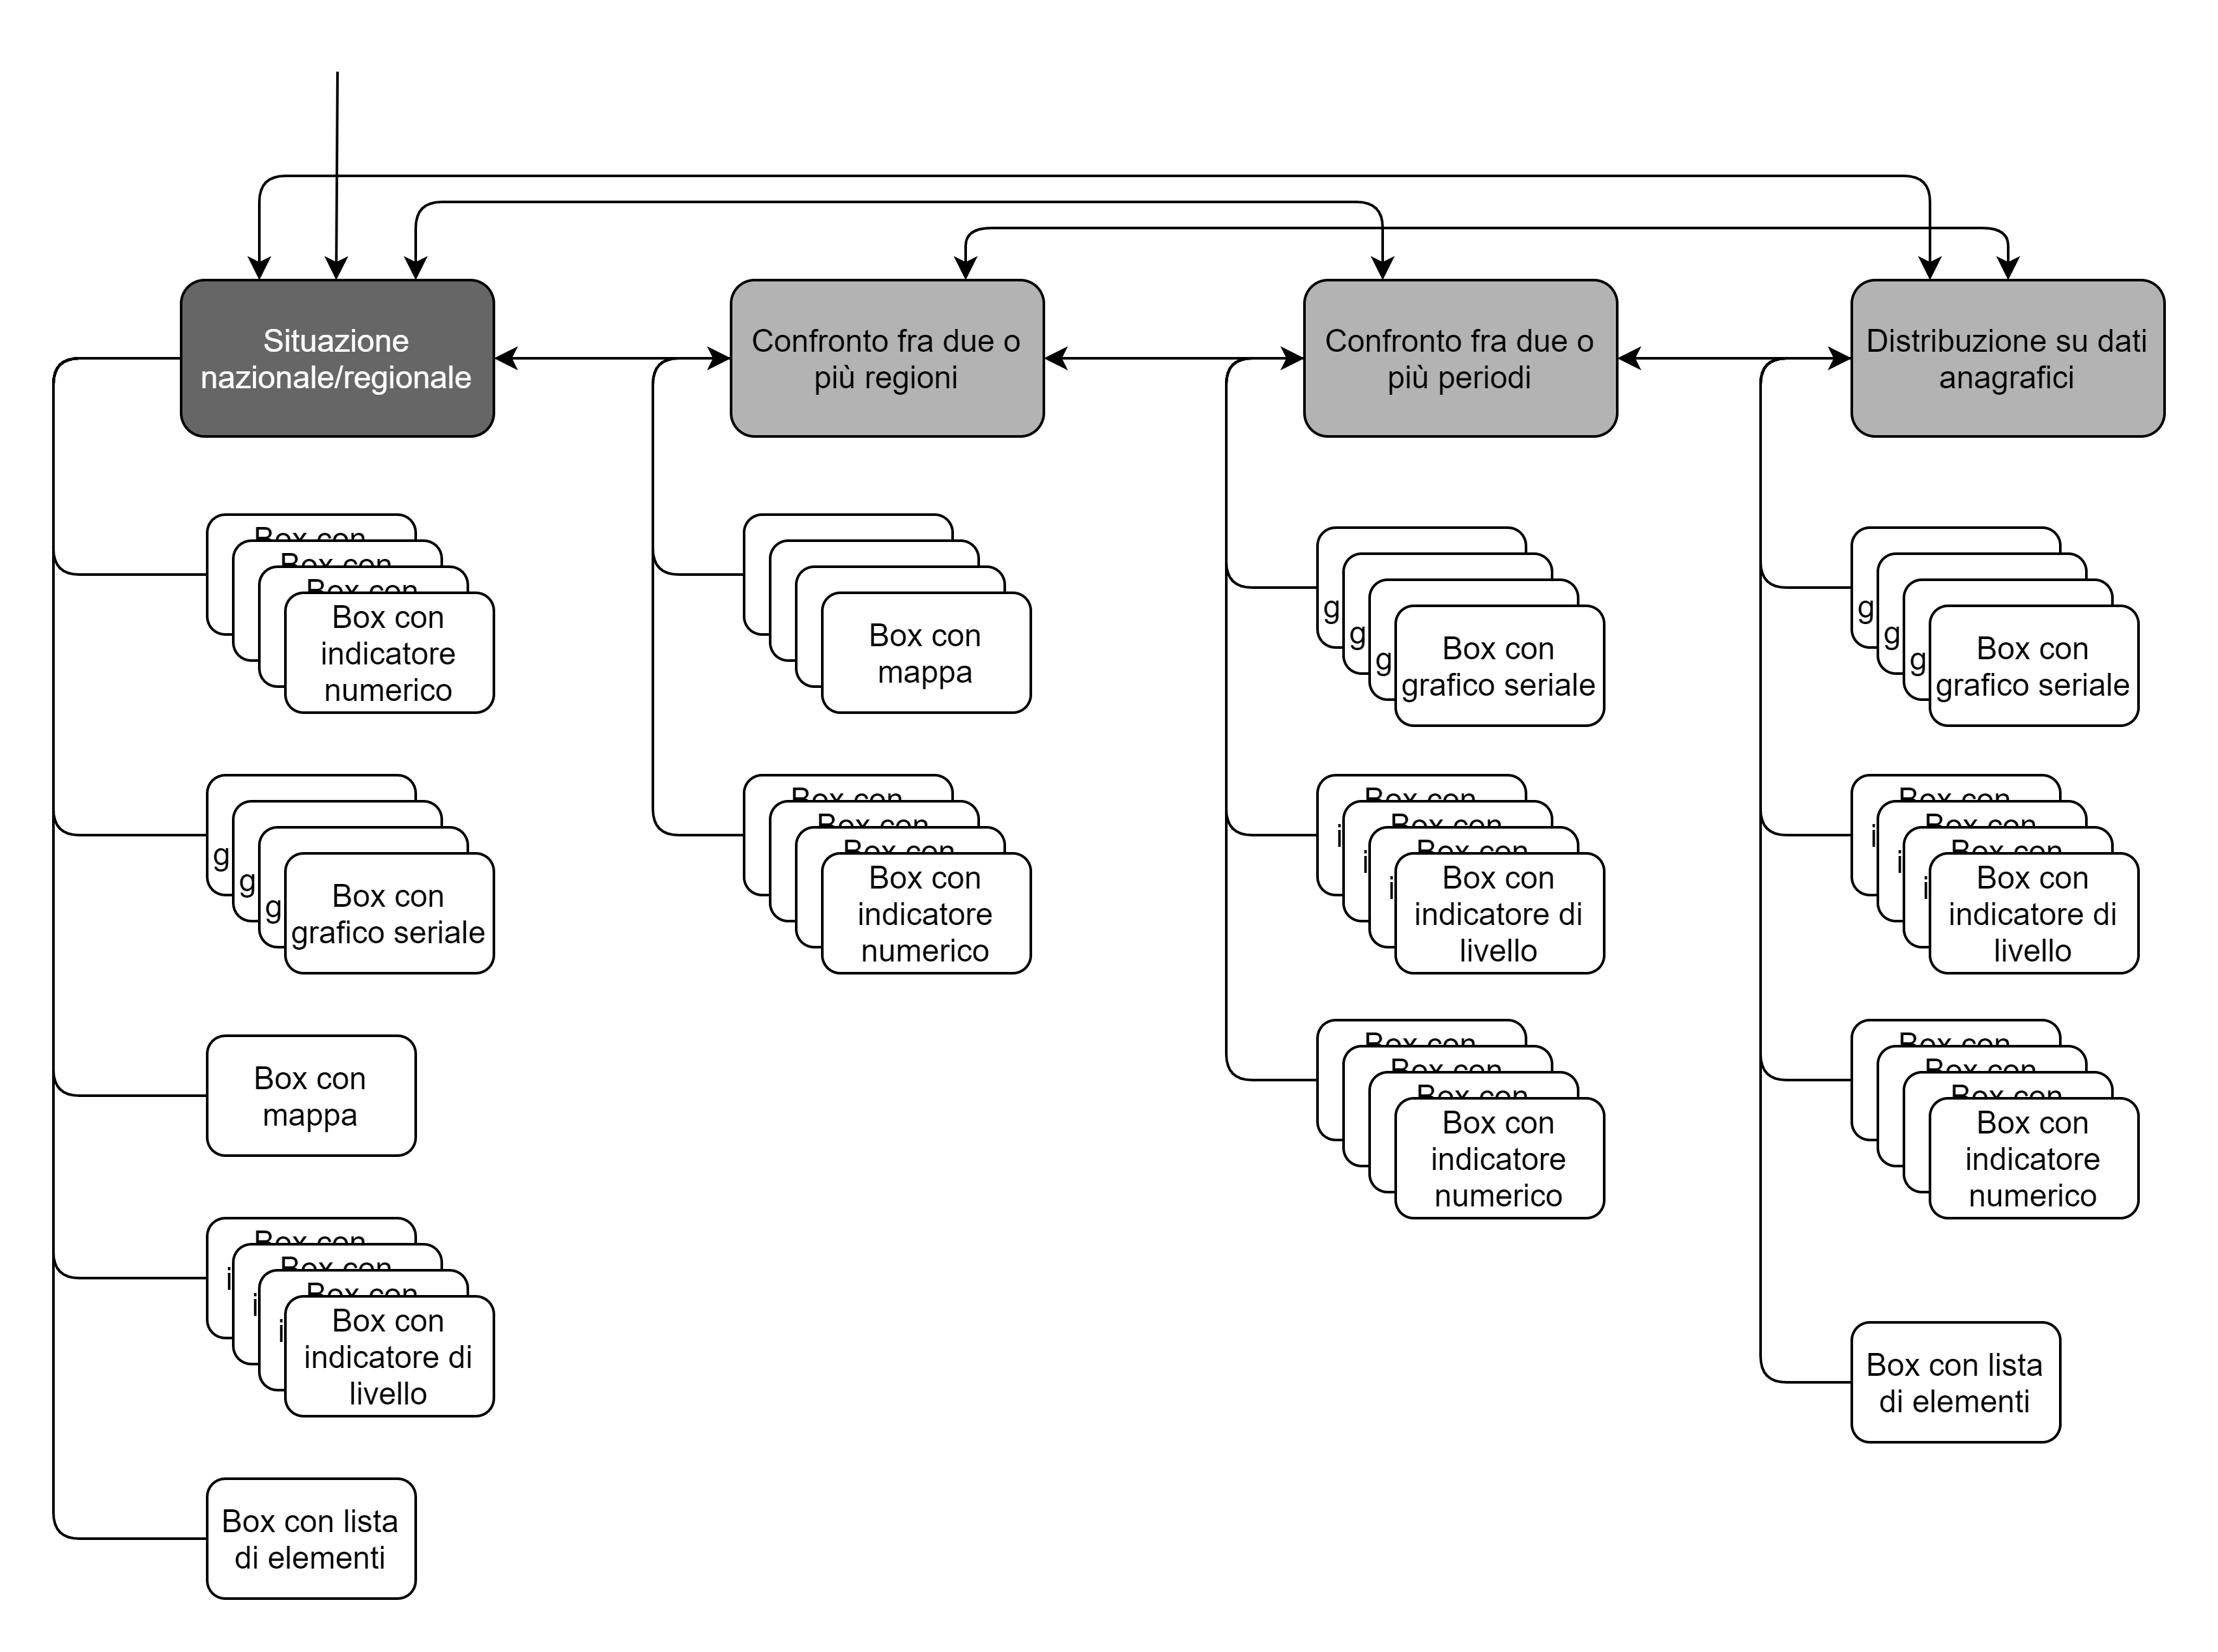
\includegraphics[width=1.0\columnwidth]{structure-blueprint/blueprint-prog-2}
    \caption{Seconda versione del blueprint per programmatori.}\label{fig:blueprint-prog-2}
\end{figure}
Questo nuovo blueprint (\ref{fig:blueprint-prog-2}) mostra come la pagina principale sia ora ``Situazione odierna (nazionale/regionale)''. Le due pagine precedentemente distinte ora, sulla base di quanto avviene nella dashboard attuale, risultano essere la medesima ma, nel caso della visualizzazione della situazione per una regione,  i dati mostrati si riferiscono a essa e non alla nazione intera grazie a una funzionalità di filtro.\\

\begin{figure}[H]
    \centering
    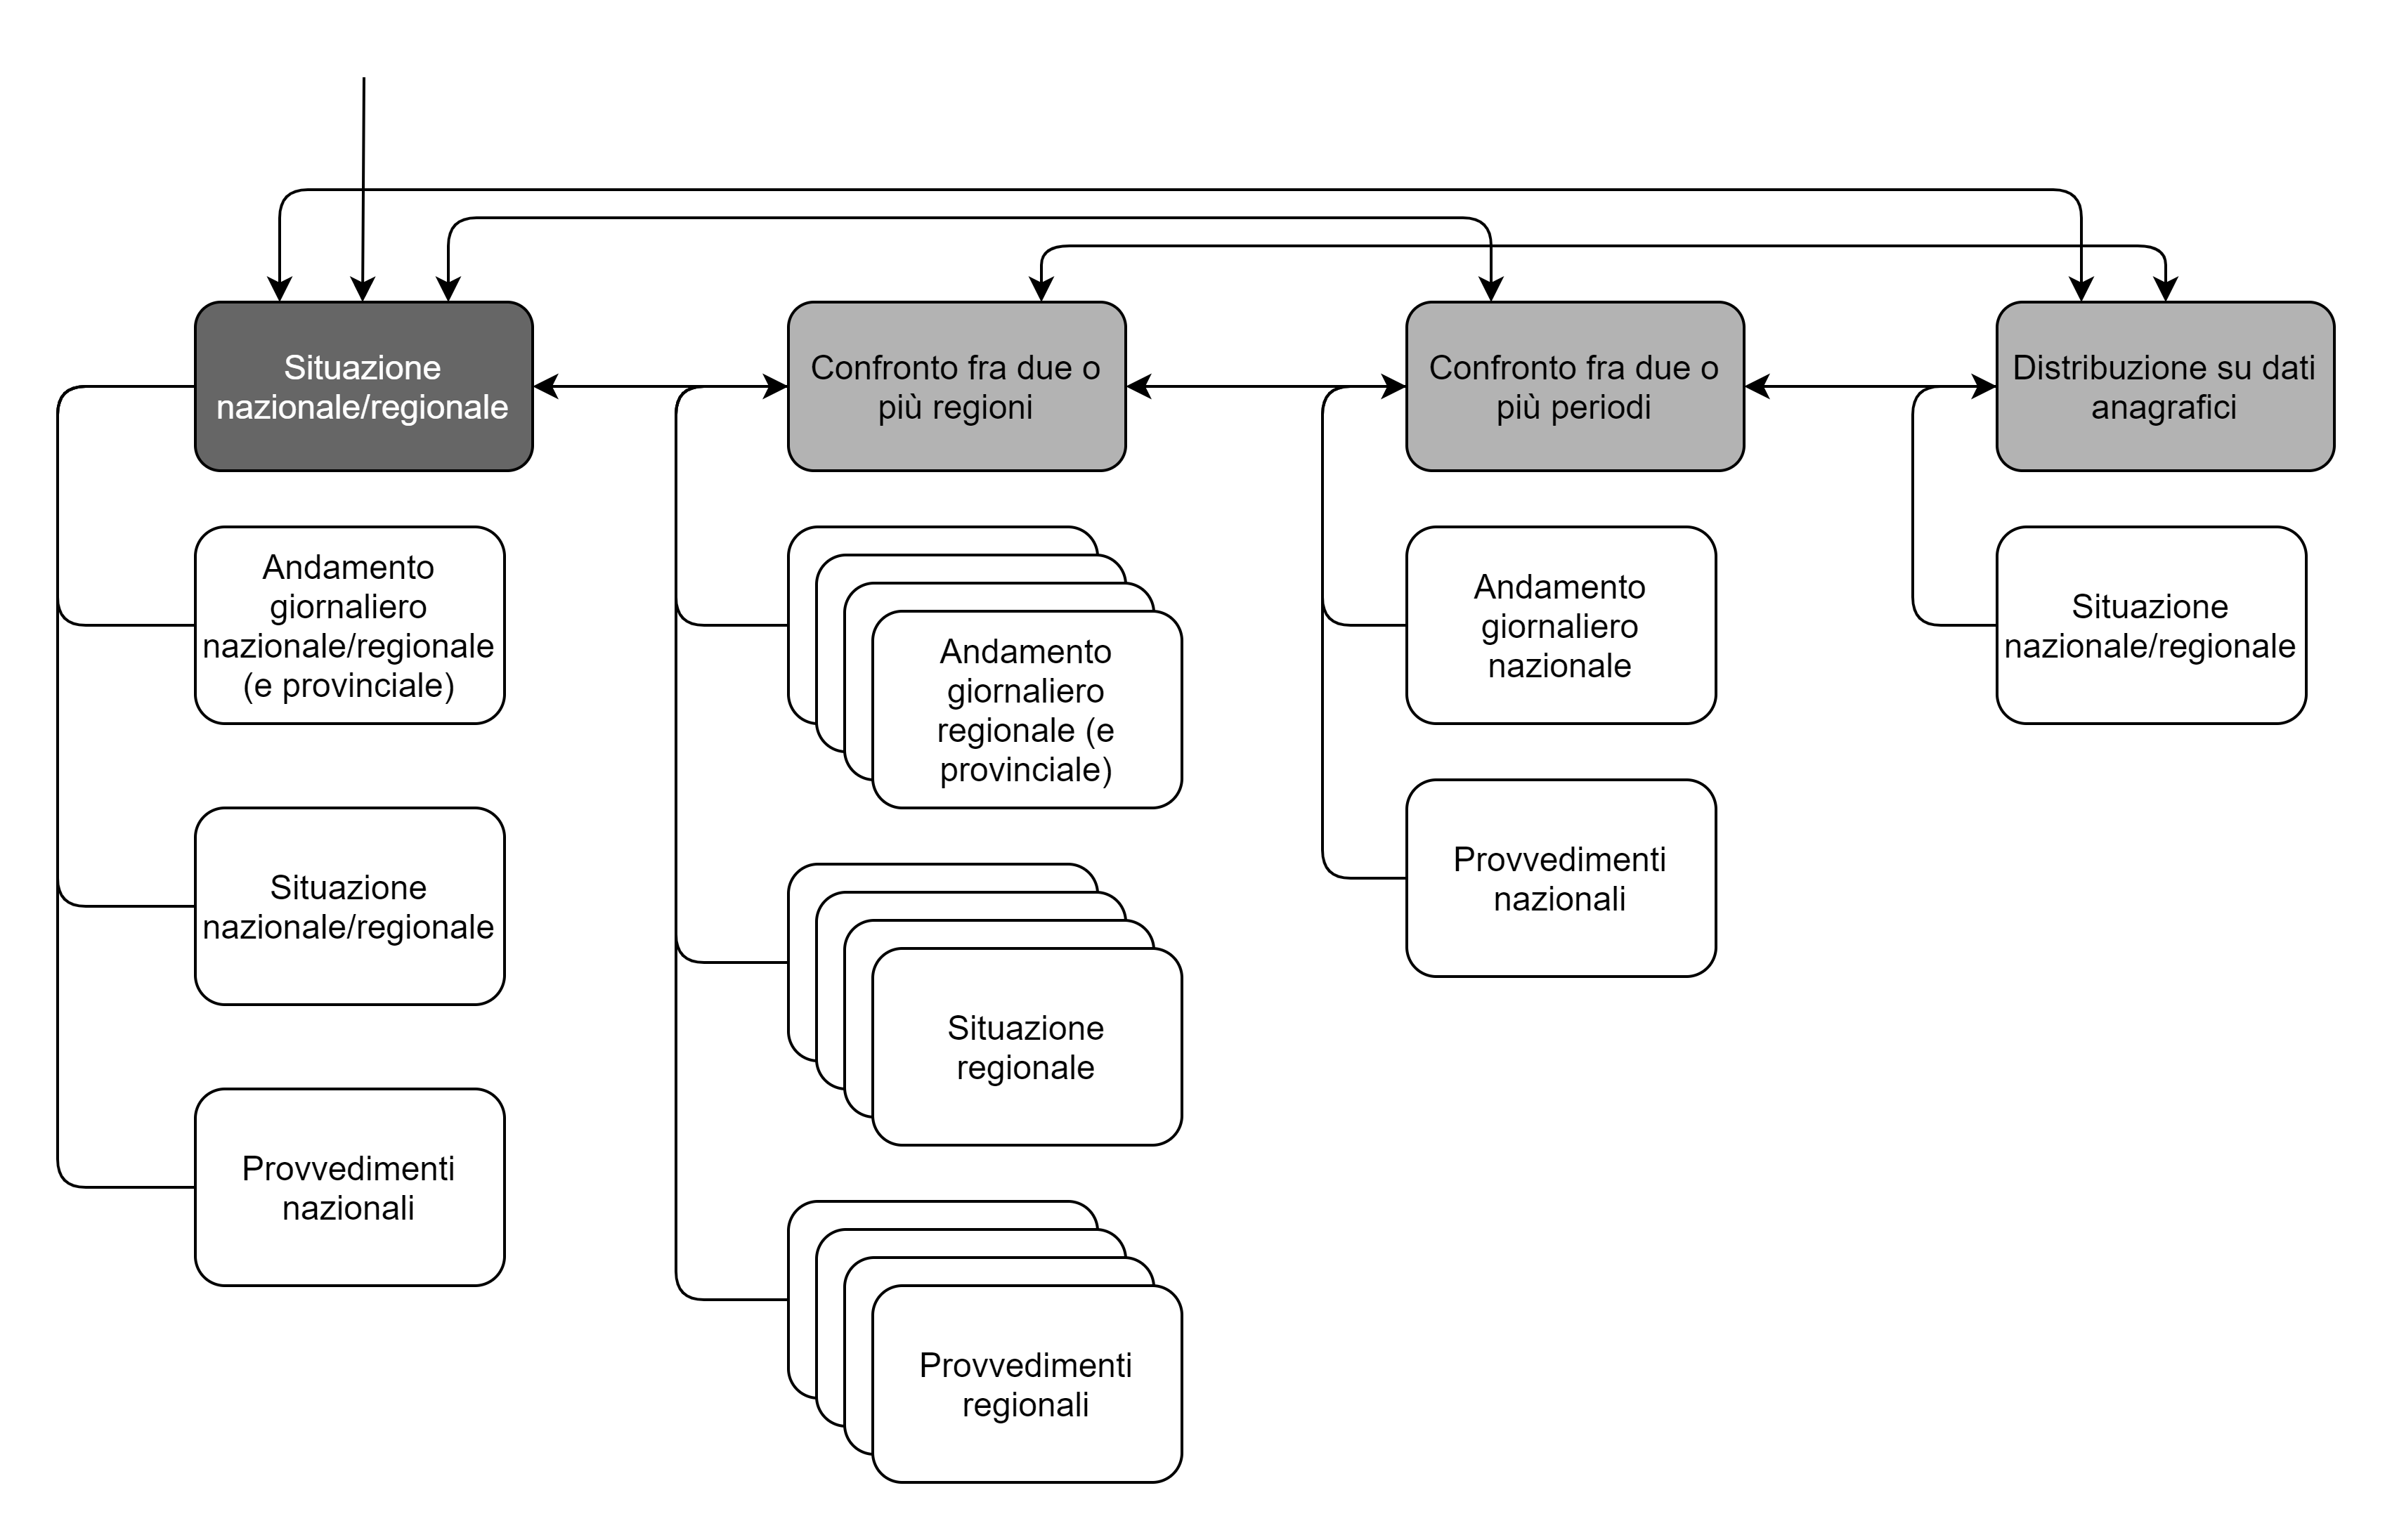
\includegraphics[width=1.0\columnwidth]{structure-blueprint/blueprint-cont-2}
    \caption{Seconda versione del blueprint per contenuti.}\label{fig:blueprint-cont-2}
\end{figure}
Per maggior chiarezza, abbiamo deciso di aggiungere anche un secondo blueprint (\ref{fig:blueprint-cont-2}) che presenti una diversa prospettiva della struttura della dashboard: in dettaglio, il nostro focus si è spostato sul comunicare i concetti che sono presenti in ogni schermata, così da fornire una più chiara e pragmatica panoramica.
Riguardo al concetto ``Andamento giornaliero'', il livello di granularità provinciale sarà presentato all'utente solo qualora si trovi a visualizzare quel concetto a livello regionale.

\subsubsection{Terza iterazione}
La terza iterazione ci ha portato alla realizzazione della versione finale dei bluprint.
\begin{figure}[H]
    \centering
    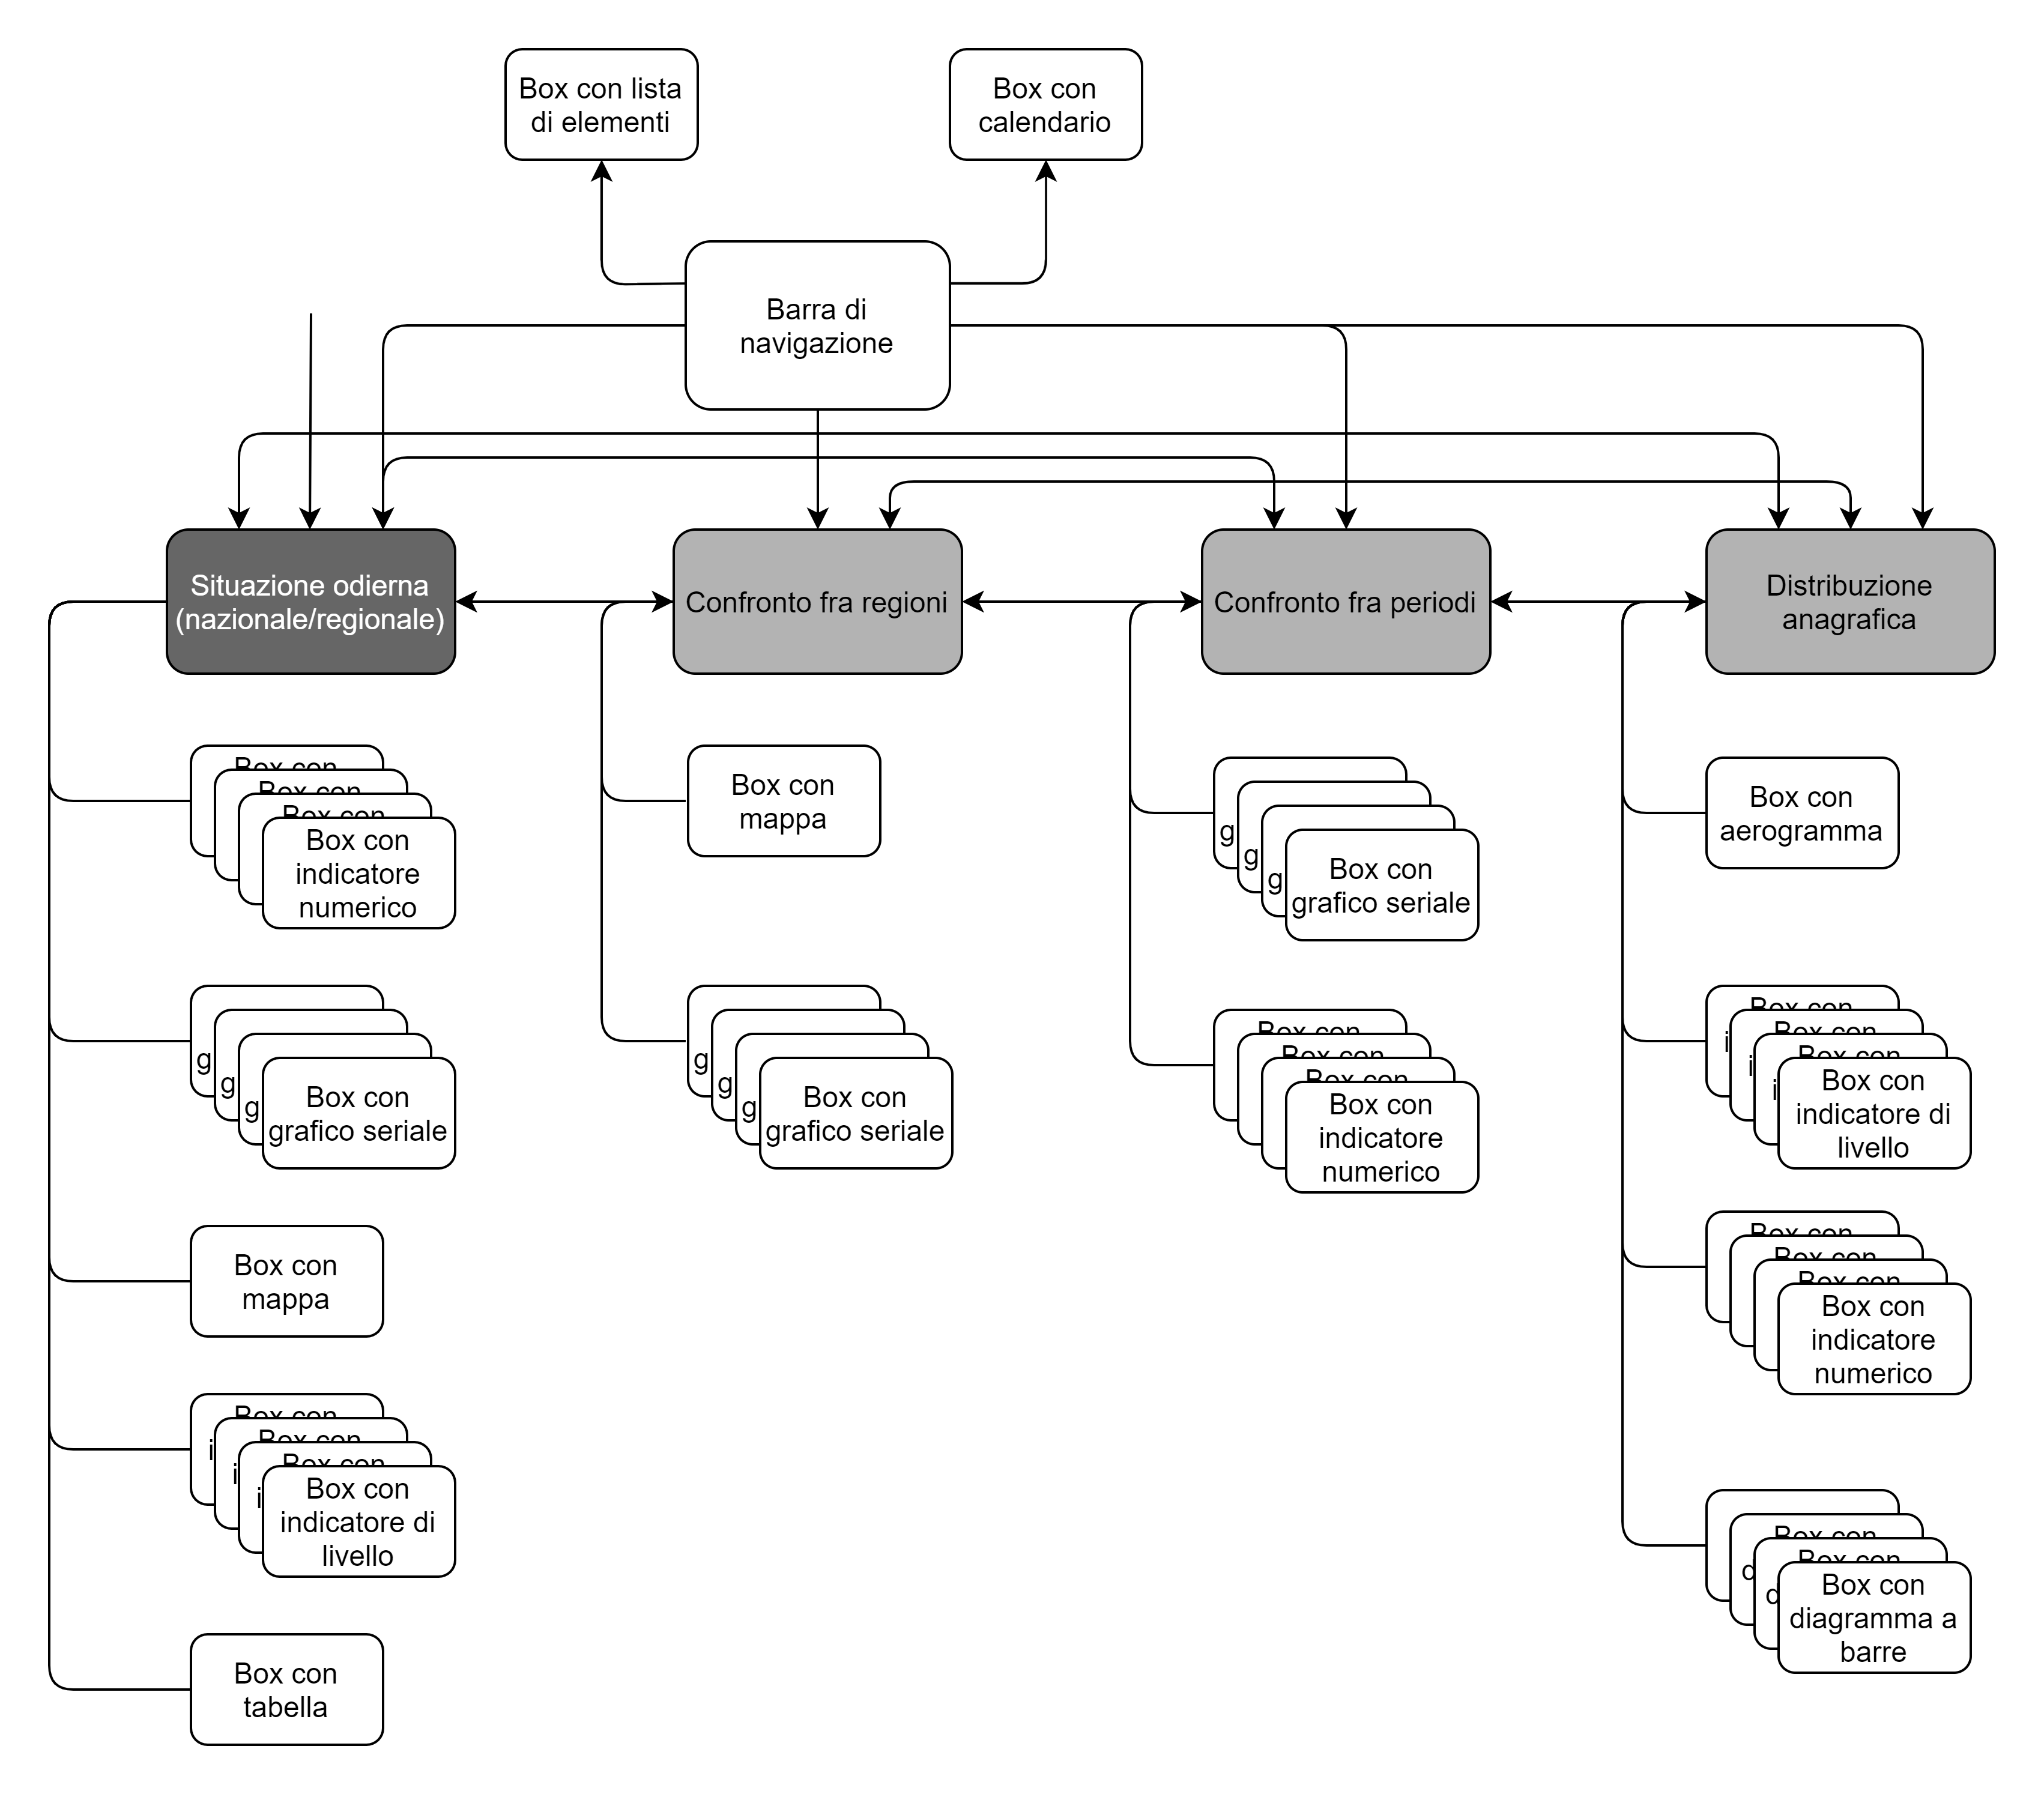
\includegraphics[width=1.0\columnwidth]{structure-blueprint/blueprint-prog-3}
    \caption{Terza versione del blueprint per programmatori.}\label{fig:blueprint-prog-3}
\end{figure}
\begin{figure}[H]
    \centering
    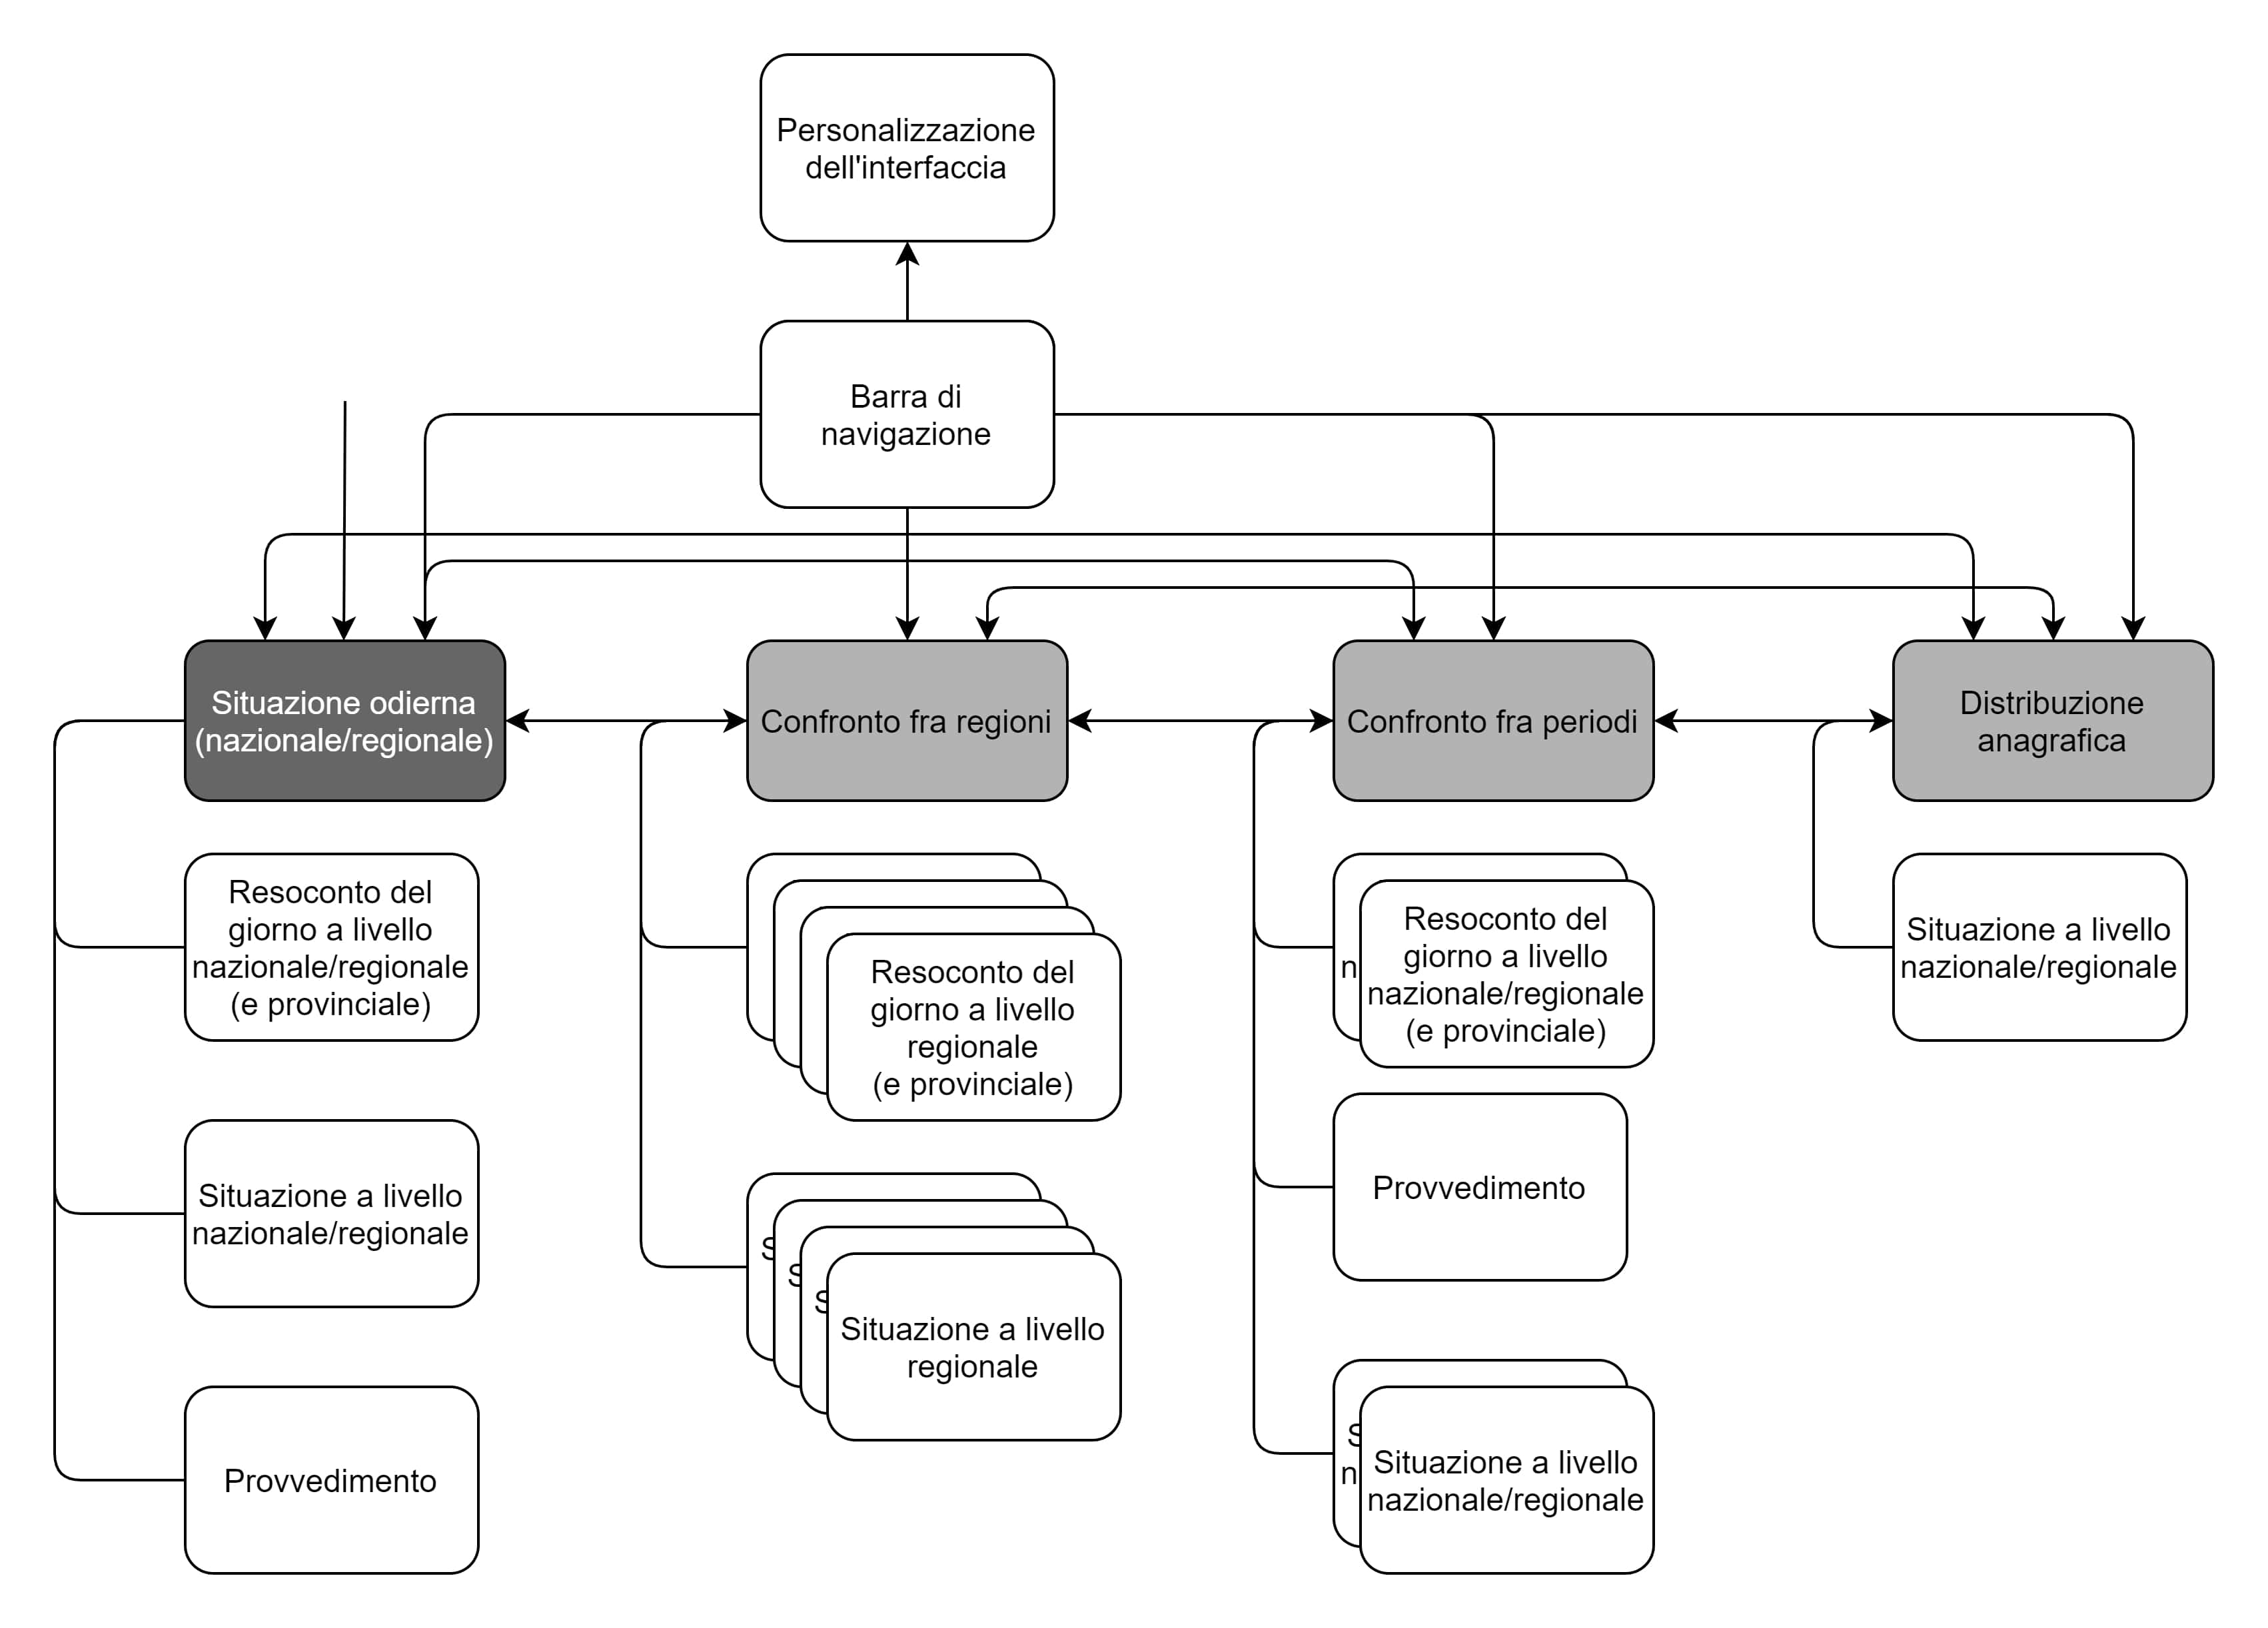
\includegraphics[width=1.0\columnwidth]{structure-blueprint/blueprint-cont-3}
    \caption{Terza versione del blueprint per contenuti.}\label{fig:blueprint-cont-3}
\end{figure}
Durante la realizzazione dei Wireframe abbiamo individuate alcune criticità nella versione due del blueprint; abbiamo quindi apportato alcune modifiche per risolvere le problematiche individuate:
\begin{itemize}
    \item abbiamo aggiunto un ``Box con calendario'' apribile mediante un bottone nella barra di navigazione;
    \item abbiamo aggiunto un ``Box con tabella'' in ``Situazione odierna'' per poter visualizzare in maniera più completa le metriche divise per regioni;
    \item abbiamo sostituito ``Box con indicatore numerico'' con  ``Box con grafico seriale'' in ``Confronto tra regioni'' per rendere più chiare le differenze tra le regioni che si vogliono analizzare;
    \item abbiamo eliminato il ``Box con indicatore di livello'' da ``Confronto tra periodi'' perché sono stati ritenuti poco opportuni;
    \item abbiamo aggiunto ``Box con areogramma'' e ``Box con diagramma a barre'' in ``Distribuzione anagrafica'' perché riteniamo siano particolarmente efficaci nel descrivere la distribuzione delle metriche.
\end{itemize}
Ancora, ci siamo ricordati del concetto ``Personalizzazione dell'interfaccia'', il quale nelle nostre intenzioni deve essere accessibile e attivabile da qualsiasi pagina, per cui lo abbiamo integrato in una barra di navigazione.
Inoltre, approssimandoci all'implementazione della dashboard, crediamo sia significativa una composizione di due task già definiti, quali il ``Confronto tra due o più periodi'' e il ``Confronto tra due o più regioni'': vogliamo che il giornalista possa filtrare i dati tanto relativamente alla dimensione temporale, quanto a quella spaziale, così da riuscire a confrontare l'andamento tra due o più regioni, in due o più periodi.
Infine abbiamo rinominato ``Andamento giornaliero'' con ``Resoconto del giorno'' in ``Situazione odierna'' perché riteniamo che questa espressione sia più chiara. 
